\documentclass[10pt]{beamer}
\usepackage{graphicx}
\usepackage{adjustbox}
\usepackage{hyperref}

\usetheme{Copenhagen}
\usecolortheme{seagull}  % You can choose from various color themes provided by metropolis
% \setbeamertemplate{footline}[frame number]
\setbeamertemplate{navigation symbols}{}

\title[WP1]{
  
\includegraphics[width=0.8\textwidth]{images/logo_Uni.png}
  Project WP1 - Vegetation}
\author[SCP]{Giulio CARPI LAPI, Pierre-Antoine SENGER}

\begin{document}

\frame{\titlepage}

\begin{frame}{Impact of vegetation on urban heat}
  \begin{figure}[h] % 'h' option tries to place the figure here
    \centering
    \includegraphics[width=1\textwidth]{images/heat_street.png}
    \caption{thermal signature of a street\cite{img:street_thermography}} % Caption for referencing
    \label{fig:heat_street} % Label for referencing
  \end{figure}
\end{frame}

\begin{frame}{Aerial thermography}
  \begin{figure}[h] % 'h' option tries to place the figure here
    \centering
    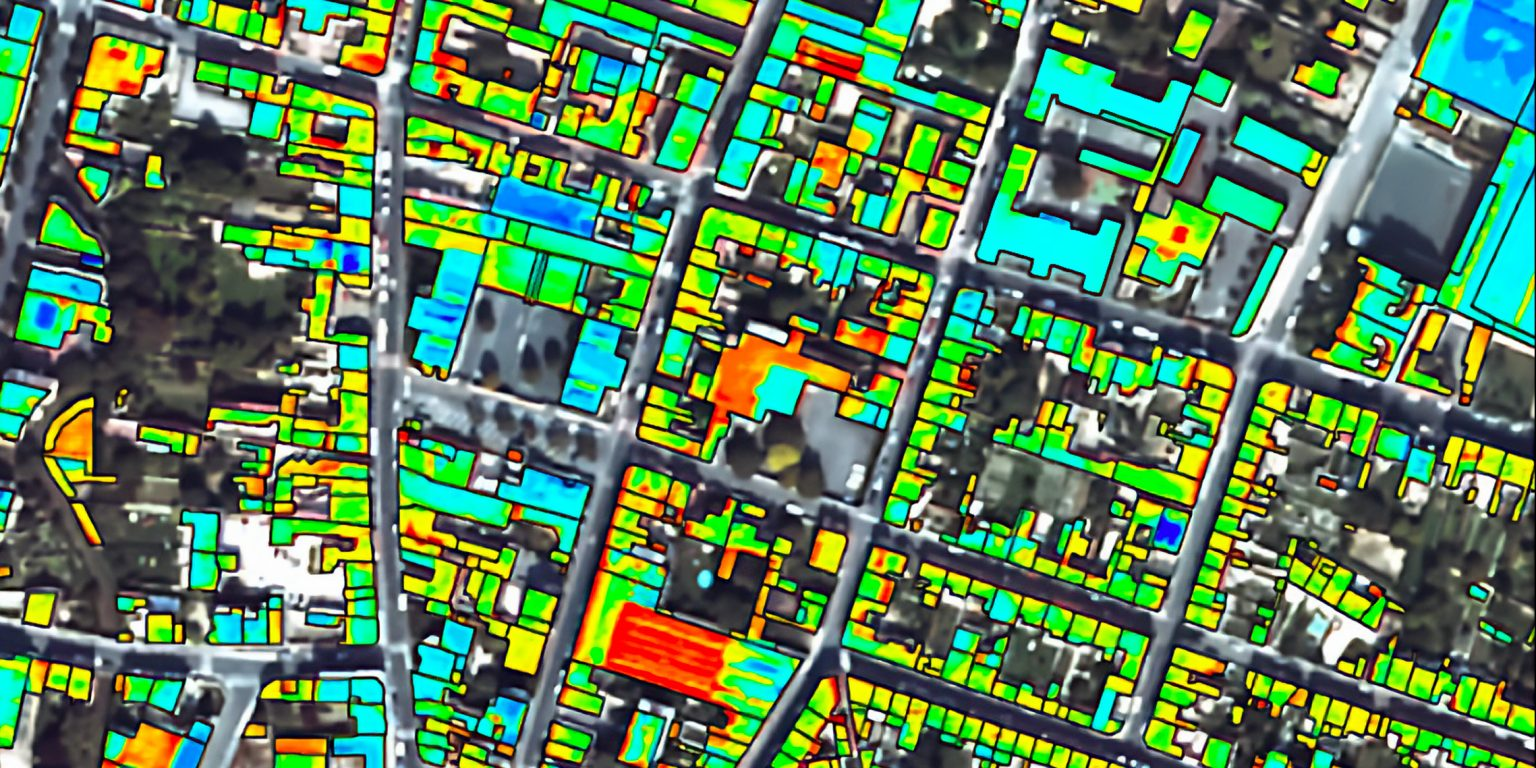
\includegraphics[width=1\textwidth]{images/thermographie-aerienne.jpg}
    \caption{aerial thermography of a city\cite{img:aerialview}} % Caption for referencing
    \label{fig:thermographie} % Label for referencing
  \end{figure}
\end{frame}

\begin{frame}{3D city model}
  \begin{figure}[h] % 'h' option tries to place the figure here
    \centering
    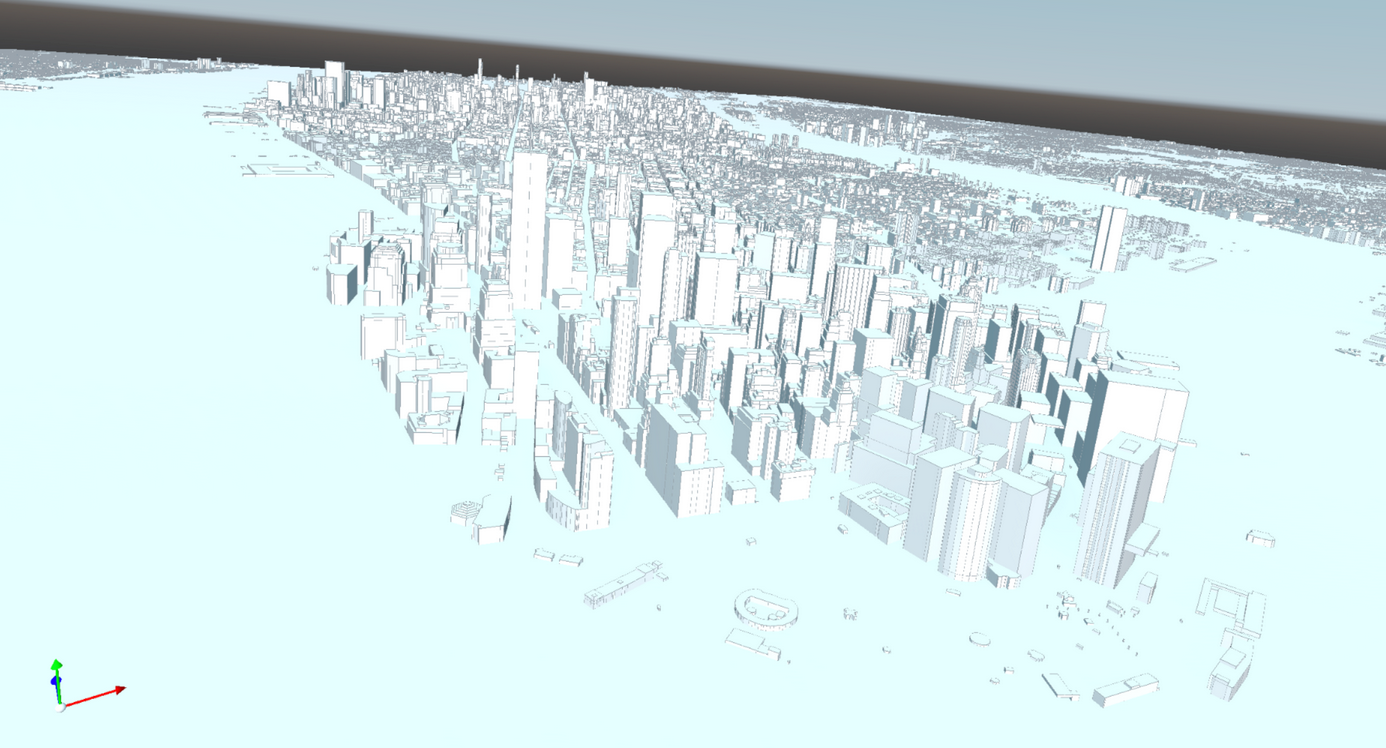
\includegraphics[width=1\textwidth]{images/NY_mesh.png}
    \caption{3D city model of New York\cite{img:NY} } % Caption for referencing
    \label{fig:city_model} % Label for referencing
  \end{figure} 
\end{frame}

\begin{frame}{Objectives}
  Main objectives : run \textbf{sun mask} and \textbf{fluid mechanics} simulations \\
  \vspace{0.5cm}

  \begin{itemize}
    \item<2-> Access the OpenStreetMap\cite{overpass} database to extract metadata:
    \begin{itemize}
      \item<3-> location of trees
      \item<4-> eight of trees
      \item <5-> type of trees
      \item <6-> etc.
    \end{itemize}
    \item<7-> Generate a C++ library of 3D tree models
    \begin{itemize}
      \item <8-> based on the metadata
      \item <9-> using CGAL\cite{cgal} C++ library 
      \item <10-> with different levels of details (LOD)
    \end{itemize}
    \item<11-> Integrate the 3D tree models into the 3D city model
  \end{itemize} 
\end{frame}

\begin{frame}{Roadmap V0}
  \begin{figure}[h] % 'h' option tries to place the figure here
    \centering
    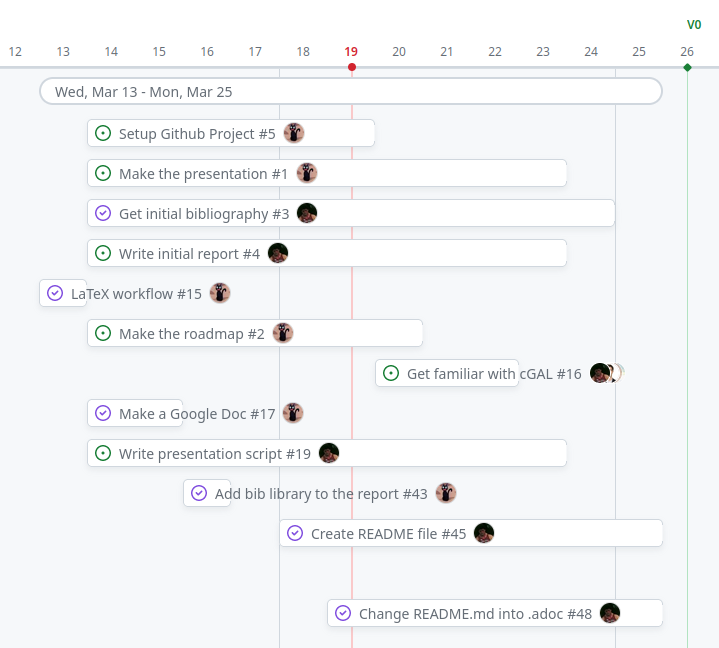
\includegraphics[width=0.8\textwidth]{images/roadmap_v0.png}
    \caption{Roadmap V0} % Caption for referencing
    \label{} % Label for referencing
    \end{figure}
\end{frame}

\begin{frame}{Roadmap V1}
  \begin{figure}[h] % 'h' option tries to place the figure here
    \centering
    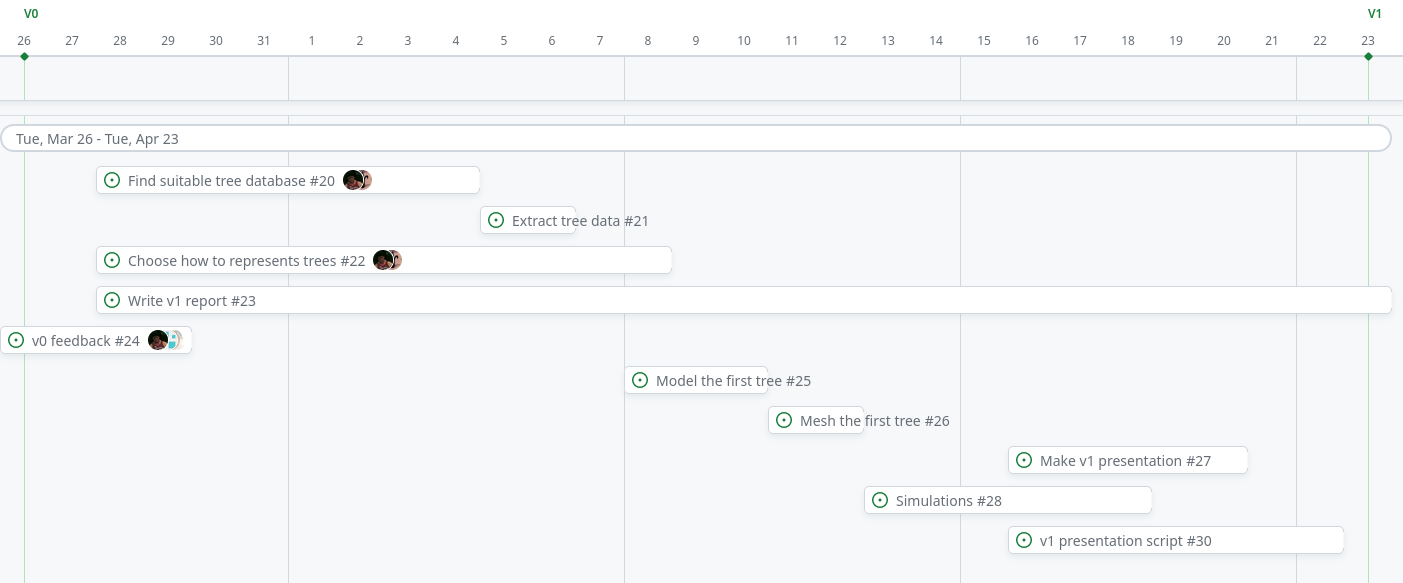
\includegraphics[width=1\textwidth]{images/roadmap_v1.png}
    \caption{Roadmap V1} % Caption for referencing
    \label{} % Label for referencing
    \end{figure}
\end{frame}

\begin{frame}{Roadmap V2}
  \begin{figure}[h] % 'h' option tries to place the figure here
    \centering
    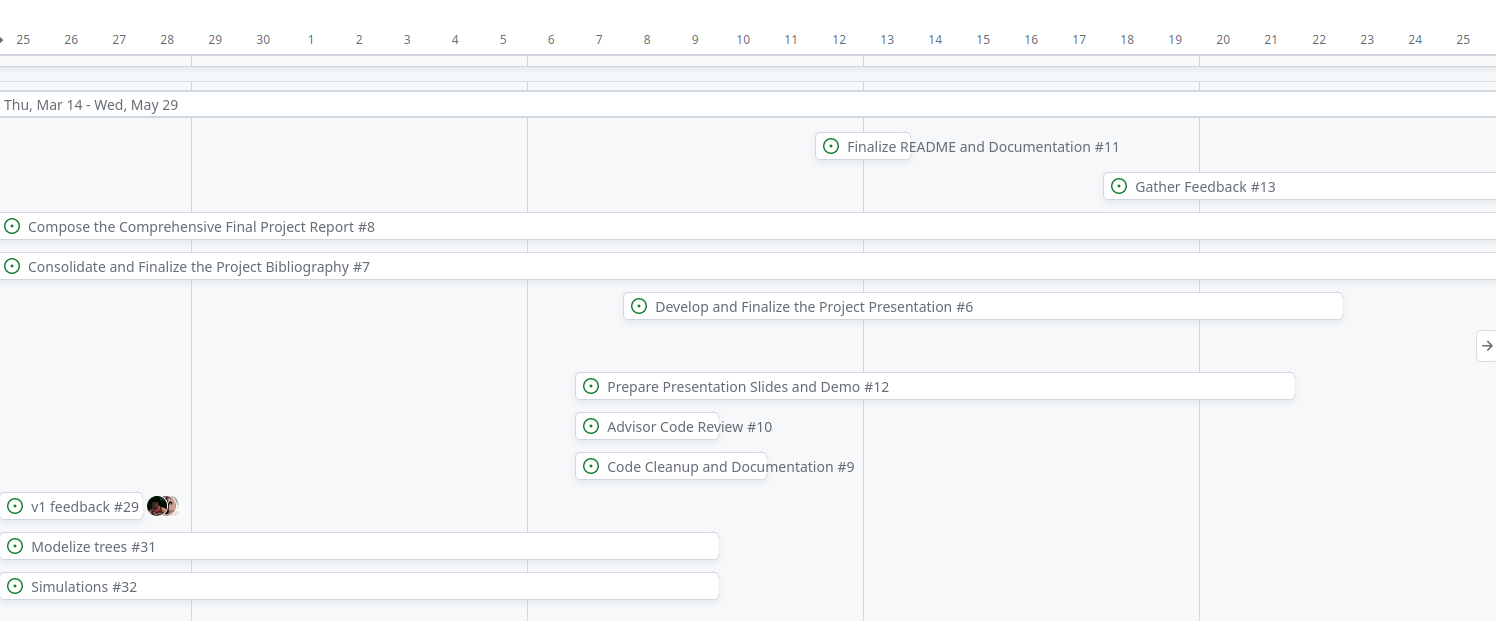
\includegraphics[width=1\textwidth]{images/roadmap_v2.png}
    \caption{Roadmap V2} % Caption for referencing
    \label{} % Label for referencing
    \end{figure}
\end{frame}


 
\nocite{*}
\bibliographystyle{plain}
\bibliography{references}

\end{document}